\subsection{Scenarios} \comment[id=K]{Add parameter notation when writing this.}
\label{subsec:appendix_scenarios}

When a country is facing a surge in infections, policy makers face the difficult decision
to weigh which instrument to apply and the extremity of each instrument. Here we
complement our analysis of the effectiveness of vaccinations and rapid tests by showing
the effects of rapid test policies vis-à-vis the more traditional NPIs, work from home
mandates and school closures. All scenarios start after Easter (April 6). Our analyses
show that many socially costly NPIs can be avoided through strong rapid testing policies.

Figure~\ref{fig:work_scenarios_detailed} shows the effects of different work policies on
the infections in the general population. We compare four scenarios with our baseline
scenario: Keeping the share of workers having physical work contacts the same as in our
baseline scenario the orange line shows what would have happened with rapid testing in
firms at the level of mid March (orange line) where only 14\% of workers regularly did
rapid tests. %
We also include a scenario what would have happened if rapid tests had become truly
mandatory after Easter\footnote{Starting on April 19th employers were required by law to
provide two weekly tests to their employees \citep{Bundesanzeiger2021}. However,
voluntarily only 60\% of workers regularly test themselves when offered tests
(\cite{Betsch2021}, 20th/21st of April).}, assuming a 95\% compliance rate on both the
employer and the employee side. On the work from home dimension we compare our baseline
scenario with 10\% more or less work from home compared to the baseline scenario. For the
total cases, the picture is very clear. Given the testing policy Germany had in place
during that time (twice weekly tests done by 35\% to 50\% of workers over that time
frame) whether 70\% (10\% below the actual mobility) or 85\% (10\% above the actual
mobility) of workers attend work physically makes little difference for the incidence. On
the other hand, the effect of a laxer or more ambitious testing policy for firms make an
important difference: As can be seen in Figure~\ref{fig:work_scenarios_newly_infected}
the gap between the two scenarios becomes quite sizable with a difference of over 80
incidence points around May 1.\comment[id=K]{Talk about detected cases?}


\begin{figure}[ht] % Work Scenarios
  \centering
  \begin{subfigure}[b]{.49\textwidth}
    \centering
    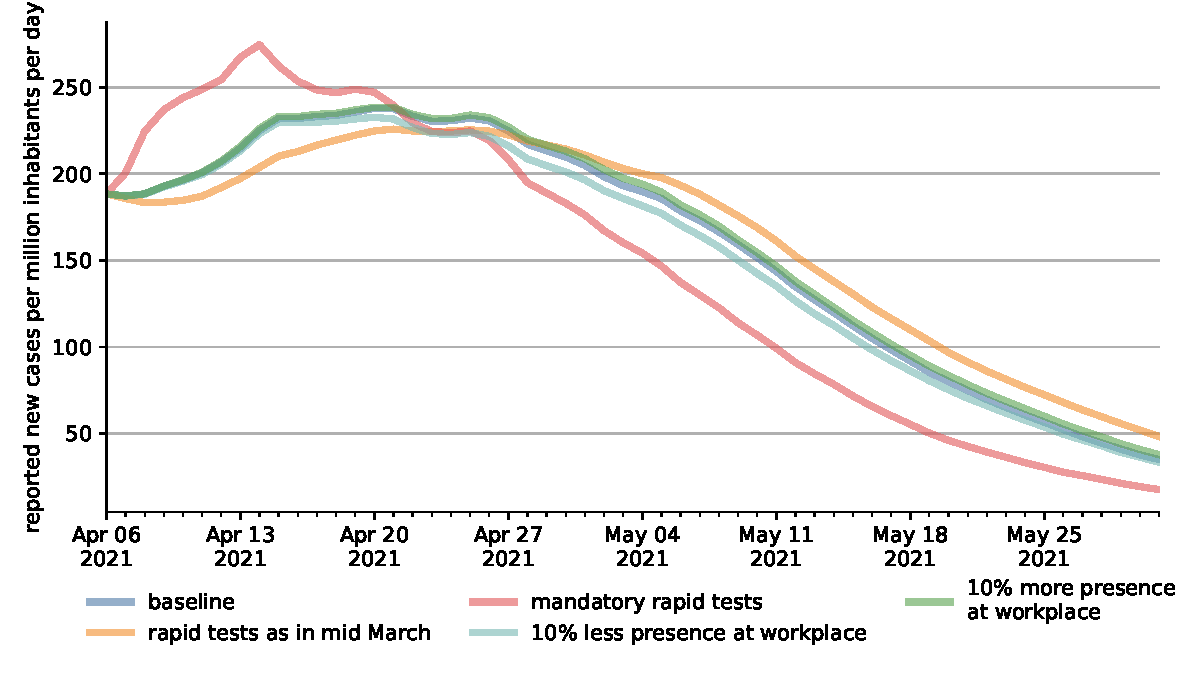
\includegraphics[width=0.9 \textwidth]{figures/results/figures/scenario_comparisons/new_work_scenarios/full_new_known_case}
    \caption{Reported Cases}
    \label{fig:work_scenarios_new_known_case}
  \end{subfigure}
  \hfill
  \begin{subfigure}[b]{.49\textwidth}
    \centering
    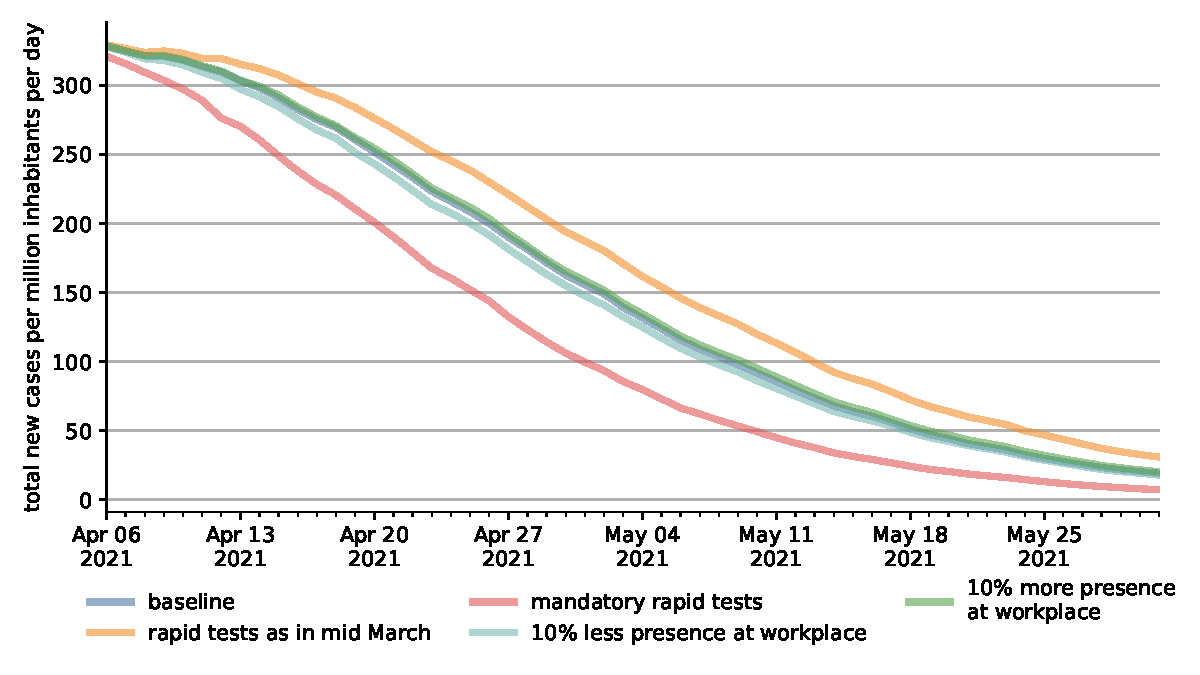
\includegraphics[width=0.9 \textwidth]{figures/results/figures/scenario_comparisons/new_work_scenarios/full_newly_infected}
    \caption{Total Cases}
    \label{fig:work_scenarios_newly_infected}
  \end{subfigure}
  \caption{The Effect of Different Work Scenarios on Reported and Total Cases}
  \label{fig:work_scenarios_detailed}
  \floatfoot{\noindent \textit{Note:} The figure shows the development of cases after
  different hypothetical policy changes take place at Easter until the end of our
  simulation period. We vary the share of workers that work from home and how many tests
  are performed at work relative to our baseline scenario. Making it mandatory to test
  all employees that do not work from home markedly reduces cases -- assuming 95\%
  compliance on both the employer and the employee side. As before, the observed cases
  can be misleading because more testing leads to more detected cases. It takes two to
  three weeks for the reduction in new infections effect to dominate the increased
  detection effect. Furthermore, the two opposing effects lead to a smaller effect size
  than is actually the case.}
\end{figure}


\FloatBarrier

The second commonly employed and also very contentious NPI we look at are school
closures. Due to the very high incidence we approximate the German schooling policy as
generous emergency care with rotating on-site schooling for graduating classes for April.
In May where cases fall and schools gradually opened, we approximate the policy as
rotating on-site schooling for most students (except for children eligible for emergency
care and graduating classes who attend in full). We compare this baseline scenario to
simply keeping schools completely closed (the brown line) and opening schools normally
(but maintaining our hygiene multiplier to account for mask wearing, ventilation etc.)
with and without tests.

As can be seen, the transmission potential in schools is very low both in the generous
emergency setting as well as the rotating operation. The difference to keeping schools
completely closed for the general population is truly negligible. Also, consistent
testing makes schools very safe to open. Would have schools opened directly after Easter
given the testing rates Germany managed at schools during that time, the total incidence
would have only been at most 14 points higher. Tests, however, are crucial here. Had
schools opened completely without any testing of students and staff, schools would have
become a driver of the pandemic with up to 50 incidence points more compared to the
baseline scenario.

\begin{figure}[ht] % School Scenarios
  \centering
  \begin{subfigure}[b]{.49\textwidth}
    \centering
    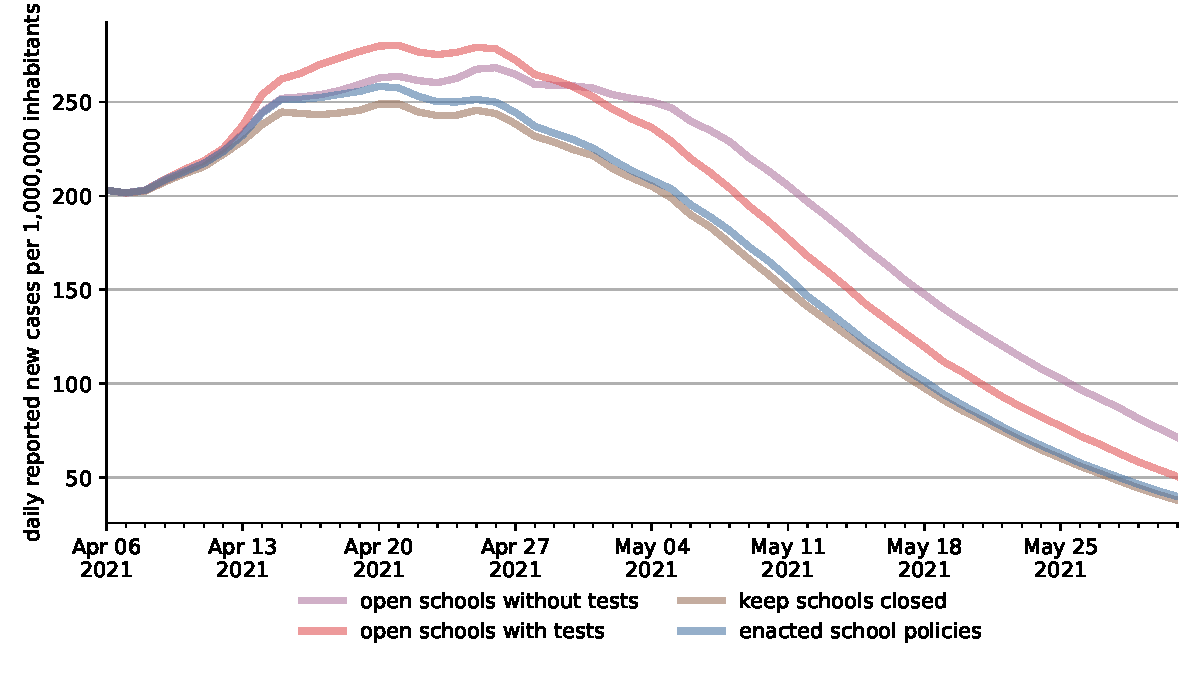
\includegraphics[width=0.9 \textwidth]{figures/results/figures/scenario_comparisons/school_scenarios/full_new_known_case}
    \caption{Reported Cases}
    \label{fig:school_scenarios_new_known_case}
  \end{subfigure}%
  \hfill
  \begin{subfigure}[b]{.49\textwidth}
    \centering
    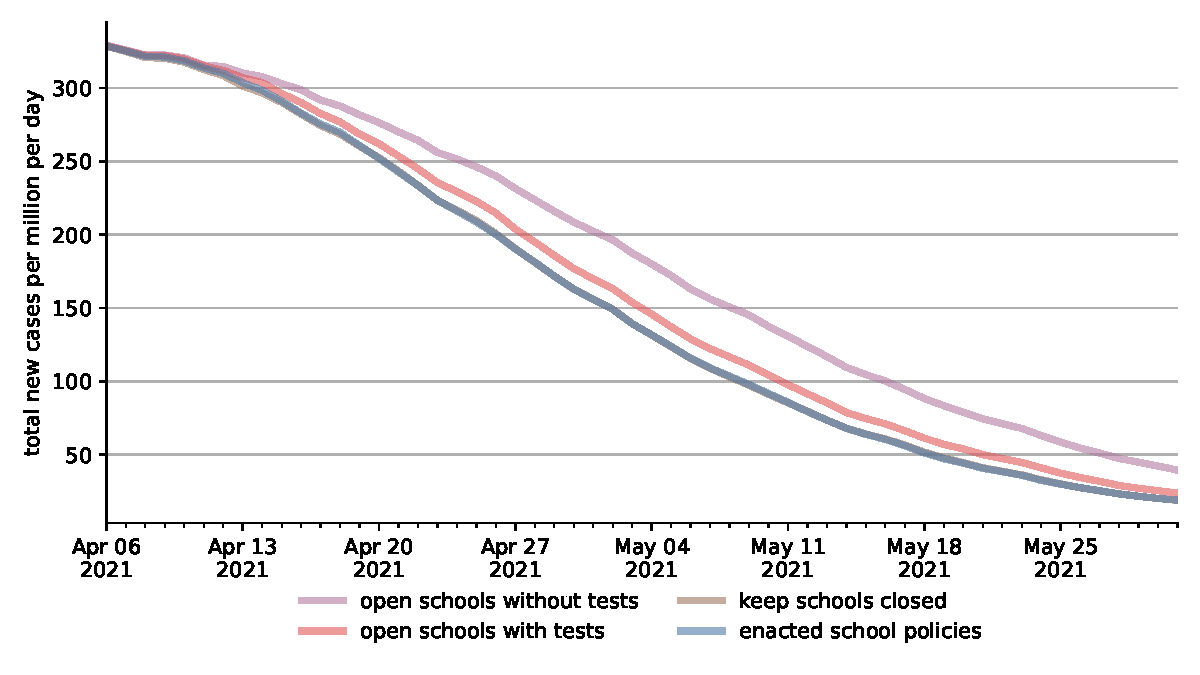
\includegraphics[width=0.9 \textwidth]{figures/results/figures/scenario_comparisons/school_scenarios/full_newly_infected}
    \caption{Total Cases}
    \label{fig:school_scenarios_newly_infected}
  \end{subfigure}
  \caption{The Effect of Different School Scenarios on Reported and Total Cases}
  \label{fig:school_scenarios_detailed}
  \floatfoot{\noindent \textit{Note:} The figure shows the development of cases after
   different hypothetical policy changes take place at Easter until the end of our
   simulation period. Apart from the enacted school policies as our baseline
   we simulate how cases would have developed if schools had been closed completely as
   the strictest possible counterfactual scenario and two opening models: One where
   schools open normally (with hygiene measures) without any testing in the education
   sector and one where schools open normally but testing shares develop as in the
   baseline scenario.
   %Our simulations suggest that the enacted policies were as effective as keeping schools
   %closed. Opening schools with the testing schemes that were in place after Easter would
   %have had a small effect on the overall incidence. However, this is mainly due to the
   %stringent testing that was in place in schools by that time. Had schools opened
   %without testing requirements the total incidence would have been up to 50 points
   %higher, though this would have been less visible in the reported cases.
   }
\end{figure}


\begin{figure}[ht] % Random Rapid Tests
  \centering
  \begin{subfigure}[b]{.49\textwidth}
    \centering
    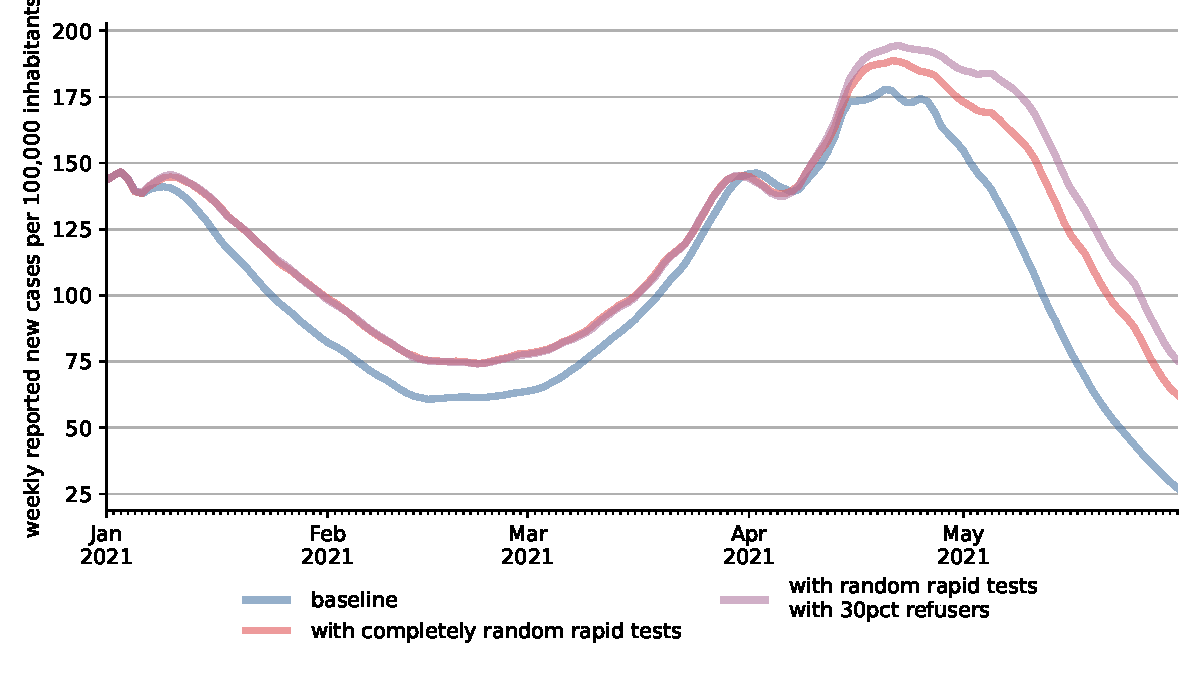
\includegraphics[width=0.9 \textwidth]{figures/results/figures/scenario_comparisons/random_rapid_tests_vs_baseline/full_new_known_case}
    \caption{Reported Cases}
    \label{fig:random_rapid_tests_new_known_case}
  \end{subfigure}%
  \hfill
  \begin{subfigure}[b]{.49\textwidth}
    \centering
    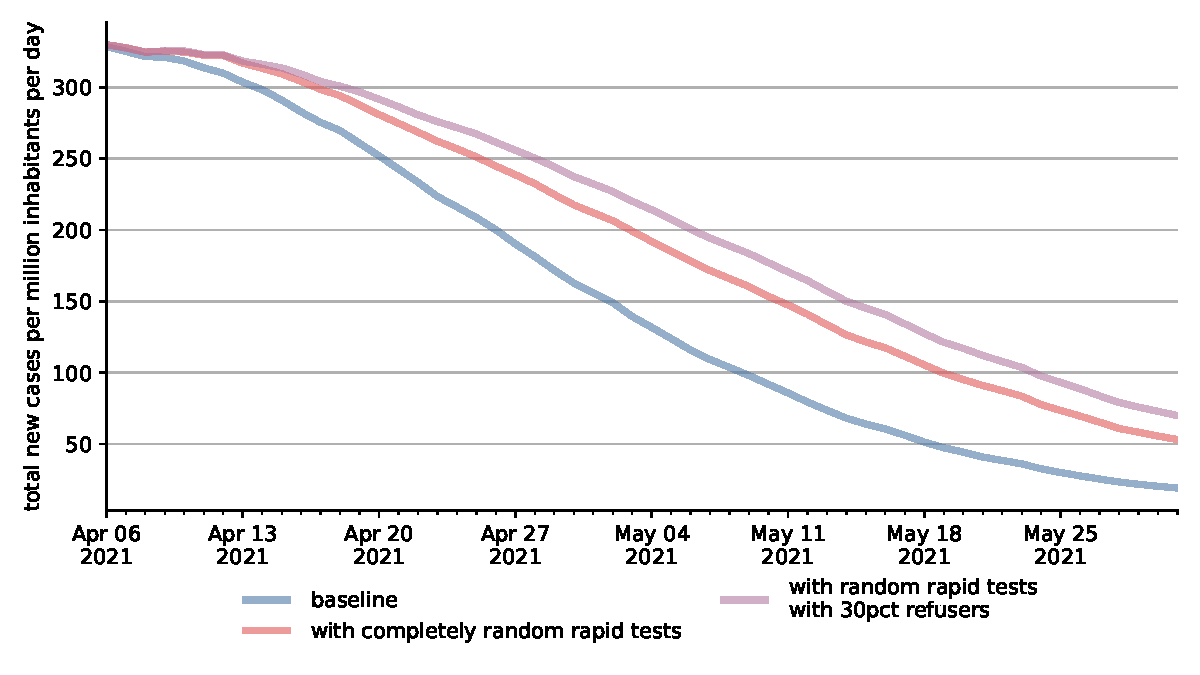
\includegraphics[width=0.9 \textwidth]{figures/results/figures/scenario_comparisons/random_rapid_tests_vs_baseline/full_newly_infected}
    \caption{Total Cases}
    \label{fig:random_rapid_tests_newly_infected}
  \end{subfigure}
  \caption{The Role of Targeted and Compliance Driven Rapid Test Demand}
  \label{fig:random_rapid_tests_detailed}
  \floatfoot{\noindent \textit{Note:} \textcolor{red}{To be written}}
\end{figure}

 \comment[id=K]{Describe that random tests are more effective at detecting cases and that
 explains the bump in the random test scenario detection in the beginning. However, cases
 fall immediately more in the non-random scenario because the targeted demand for tests
 by household members leads to a much more efficient interruption of infection chains
 because we catch the household members very early in their infectious period.}

 \comment[id=K]{Write that at the end of our simulation period nearly everyone in the
 educ sector did rapid tests because they are mandatory but still 40-50\% refusers in the
 work and private sector}

\FloatBarrier
